\documentclass[A4,12PT, english, twocolumn]{journal}
\usepackage{amsmath,amssymb,amsfonts}
\usepackage[margin=0.7in]{geometry}
\usepackage{graphicx}
\usepackage{enumitem}
\usepackage{xcolor}
\usepackage{hyperref}
\usepackage{tabularray}
\usepackage{multicol}
\usepackage{tikz}
\usepackage{circuitikz}
\usepackage{scalerel}
\usepackage{pict2e}
\usepackage{tkz-euclide}
\usetikzlibrary{calc}
\usetikzlibrary{patterns,arrows.meta}
\usetikzlibrary{shadows}
\usetikzlibrary{external}

%pgfplots
\usepackage{pgfplots}
\pgfplotsset{compat=newest}
\usepgfplotslibrary{statistics}
\usepgfplotslibrary{fillbetween}

\def\infinity{\rotatebox{90}{8}}

% Hiperlink
\hypersetup{
    colorlinks=true,
    linkcolor=blue,
    filecolor=magenta,      
    urlcolor=cyan,
    pdftitle={Overleaf Example},
    pdfpagemode=FullScreen,
}
%\usepackage{style}
\NewDocumentCommand{\Log}{o}{%
\IfNoValueTF{#1}{}{{}^{#1}\!}\log}%
  
%command buat logaritma dengan basisnya di pojok kiri
%\textheight=17cm
%\textwidth=10cm
%\usepackage{blindtext}
\setenumerate[1]{itemsep=0,5cm}
\setenumerate[2]{topsep=5pt, itemsep=5pt, label=\textbf{\Alph*}.}

\title{Matematika Saintek \& Fisika UTUL UGM 2018 Kode 576}
\author{Fauzan Akbar Sukandar Putra \\ \LaTeX}

\begin{document}

\maketitle

%\begin{minipage}{0.5\textwidth}
\begin{enumerate}
%1%
\item Suatu deret geometri tak hingga mempunyai jumlah $\frac{9}{4}$. Suku pertama dan rasio deret tersebut masing-masing $a$ dan $- \frac{1}{a}$, dengan $a>0$. Jika $U_n$ menyatakan suku ke-$n$ pada deret tersebut, maka $3U_6-U_5=$ \dots
    \begin{enumerate}
        \item $0$
        \item $\frac{2}{27}$
        \item $-\frac{2}{27}$
        \item $\frac{1}{27}$
        \item $-\frac{1}{27}$
    \end{enumerate}
  
%2%
\item Diketahui $m$ adalah sisa pembagian polinomial \\ $h \left(x \right) = x^3-x^2+2x+2$ oleh $x-1$. Nilai $k$ yang memenuhi $\lim\limits_{x \longrightarrow \infinity} {\left(\frac{mx^3-kx+5}{kx^3+3x^2-7}-k \right) = 0}$ adalah \dots
    \begin{enumerate}
        \item $-1$
        \item $0$
        \item $\frac{1}{2}$
        \item $1$
        \item $2$
    \end{enumerate}
     
%3%  
\item Jika fungsi $f$ dengan $f \left(x \right) = \sqrt[3]{x^3+m^3x^6}$, turun pada $\left(-\infinity, -1 \right]$, maka $8m^3+8=$ \dots
    \begin{enumerate}
        \item $16$
        \item $12$
        \item $8$
        \item $4$
        \item $0$
    \end{enumerate}
   
%4% 
\item Pertidaksamaan $^2\Log{\left(x^2-x \right)} \leq 1$ mempunyai penyelesaian \dots
    \begin{enumerate}
        \item $x<0$ atau $x>1$
        \item $-1<x<2 \; ; x \neq 1, \; x \neq 0$
        \item $-1 \leq x<0$ atau $1<x \leq 2$
        \item $-1 \leq x \leq 0$ atau $1 \leq x \leq 2$
        \item $-1<x<0$ atau $1 \leq x < 2$
    \end{enumerate}

%5%
\item Jika bilangan bulat $p$ merupakan akar $f \left(x \right) = 0$ dengan $f \left(x \right) = px^2-3x-p-3$, maka gradien garis singgung kurva $y= f \left(x \right)$ di titik dengan absis $x=p$ adalah \dots
    \begin{enumerate}
        \item $-5$
        \item $-3$
        \item $-1$
        \item $3$
        \item $5$
    \end{enumerate}
    
%6%
\item Jika $x>y \geq 1$ dan
\begin{ceenter}
    $\Log{\left(x^2+y^2+2xy \right)} = 2 \Log{\left(x^2-y^2 \right)}$. \\
\end{ceenter}
Maka $^x\Log{\left(1+y \right)} =$ \dots
    \begin{enumerate}
        \item $\Log{2}$
        \item $-1$
        \item $-\frac{1}{2}$
        \item $\frac{1}{2}$
        \item $1$
    \end{enumerate}
    
%7%  
\item Akar-akar persamaan $x^2+px+27=0$ adalah $x_1$ dan $x_2$ yang semuanya positif dan $x_2>x_1$. Jika $x_1, \; x_2,$ dan $5x_1$ berturut-turut suku pertama, suku ke dua, dan suku ke tiga barisan aritmatika, maka suku ke sepuluh adalah \dots
    \begin{enumerate}
        \item $55$
        \item $57$
        \item $59$
        \item $61$
        \item $63$
    \end{enumerate}
    
%8%  
\item Diberikan lingkaran pada bidang koordinat yang memotong sumbu-$X$ di $\left(1,0 \right)$ dan $\left(3,0 \right)$. Jika lingkaran tersebut menyinggung sumbu-$Y$, maka titik singgung yang mungkin adalah \dots
    \begin{enumerate}
        \item $\left(0,1 \right)$
        \item $\left(0,2 \right)$
        \item $\left(0, \sqrt{3} \right)$
        \item $\left(0, \sqrt{5} \right)$
        \item $\left(0,3 \right)$
    \end{enumerate}
    
%9%  
\item Diketahui segitiga $ABC$ dengan $\left|BC \right| = 2\sqrt{3}$ dan $\angle BAC = 60^{\circ}$. Jika $\left|AC \right| + \left|AB \right| = 6$, maka $\left|{\left|AC \right| - \left|AB \right|}\right| =$ \dots
	\begin{enumerate}
		\item $\frac{1}{2}$
		\item $1$
		\item $\frac{3}{2}$
		\item $2$
		\item $\frac{5}{2}$
	\end{enumerate}
	
%10%
\item Diketahui proyeksi vektor $v$ pada vektor $u$ sama dengan proyeksi vektor $w$ pada vektor $u$. Jika $2v \cdot u = \sqrt{3}\left|v \right| \left|u \right|$ dan $2w \cdot u = \left|w \right| \left|u \right|$, maka $\frac{v \cdot w}{\left|v \right| \left|w \right|} =$ \dots
   \begin{enumerate}
        \item $\frac{1}{2}$
        \item $\frac{1}{2} \sqrt{2}$
        \item $\frac{1}{2} \sqrt{3}$
        \item $1$
        \item $\frac{1}{2} \sqrt{5}$
   \end{enumerate}
   
%11%
\item Diketahui $P_1$ adalah pencerminan titik $P\left(2,k \right)$ terhadap garis $y=x$. Jika luas segitiga $POP_1$ adalah 6, \\ maka $\left|k \right| =$ \dots
    \begin{enumerate}
        \item $2 \sqrt{2}$
        \item $2 \sqrt{3}$
        \item $\sqrt{10}$
        \item $4$
        \item $16$
    \end{enumerate}
  
%12% 
\item Jika $\left(p,q \right)$ merupakan titik puncak grafik fungsi \\ $f \left(x \right) = ax^2+2ax+a+1$, dengan $f \left(a \right) = 19$, \\ maka $p+2q+3a =$ \dots
    \begin{enumerate}
        \item $7$
        \item $6$
        \item $0$
        \item $-1$
        \item $-2$
    \end{enumerate}
    
%13% 
\item Diberikan suku banyak $p \left(x \right) = ax^3+bx^2+a$ dengan \\ $a \neq 0$. Jika $x^2+nx+1$ merupakan faktor $p \left(x \right)$, \\ maka $n =$ \dots
    \begin{enumerate}
        \item $-3$
        \item $-2$
        \item $-1$
        \item $1$
        \item $3$
    \end{enumerate}

%14% 
\item Suku banyak
\begin{center}
    $P \left(x \right) = ax^5+x^4+bx^3+x^2+cx+d$
\end{center} \\
berturut-turut bersisa $3$ dan $-7$ ketika dibagi $x+1$ dan $x-1$. Sisa pembagian $P \left(x \right)$ oleh $x$ adalah \dots
\begin{enumerate}
        \item $-4$
        \item $-2$
        \item $0$
        \item $2$
        \item $4$
    \end{enumerate}

%15% 
\item Jumlah suatu deret geometri tak hingga adalah $10$, dan jumlah suku-suku bernomor ganjil adalah $6$. Suku ke-$2$ deret tersebut adalah \dots
    \begin{enumerate}
        \item $\frac{20}{3}$
        \item $\frac{20}{6}$
        \item $\frac{20}{9}$
        \item $\frac{20}{11}$
        \item $\frac{20}{13}$
    \end{enumerate}
    

%FISIKA %
%16%
\newpage
\item Sebuah benda bergerak di suatu permukaan yang kasar dengan koefisien gesek antara permukaan dengan benda konstan $\mu$. Bila awalnya energi kinetik benda adalah $E$ dan jarak yang dapat ditempuh benda sebelum berhenti adalah $x$ maka besar massa benda adalah \dots
    \begin{enumerate}
        \item $\frac{3E}{g \mu x}$
        \item $\frac{E}{2 g \mu x}$
        \item $\frac{2E}{g \mu x}$
        \item $\frac{E}{g \mu x}$
        \item $\frac{E}{4 g \mu x}$
    \end{enumerate}
  
%17%
\item Sebuah partikel ditembakkan dari ketinggian $h$ dari tanah. Jika massa partikel $m$ dan percepatan gravitasi $g$, hitunglah kecepatan awal yang harus diberikan kepada partikel tersebut agar pada saat mencapai ketinggian $2h$ diatas tanah, energi kinetiknya lenyap!
    \begin{enumerate}
        \item $\sqrt{\frac{2g}{h}}$
        \item $\sqrt{gh}$
        \item $\sqrt{2gh}$
        \item $\sqrt{\frac{gh}{2}}$
        \item $\sqrt{\frac{2h}{g}}$
    \end{enumerate}
     
%18%
\item Sebuah kapal mengambang di permukaan air laut dengan sebagian volume kapal tadi di bawah permukaan air. Massa total kapal adalah $100 \; ton$, maka volume kapal yang berada di bawah permukaan air adalah \dots $m^3$
\textbf{(anggap massa jenis air laut $1,0 \; g/cm^3$)}
    \begin{enumerate}
        \item $100$
        \item $1000$
        \item $10.000$
        \item $100.000$
        \item $1.000.000$
    \end{enumerate}
   
%19% 
\item Sebuah pegas ringan memiliki tetapan pegas $500 \; N/m$. Salah satu ujung pegas itu diikat pada balok yang terletak di lantai yang cukup licin, sedangkan ujung yang lain ditarik (lihat gambar) sehingga balok mengalami percepatan $20 \, m/s^2$. Jika massa balok $1 \; kg$, berapakah energi potensial pegas? 
\begin{center}
    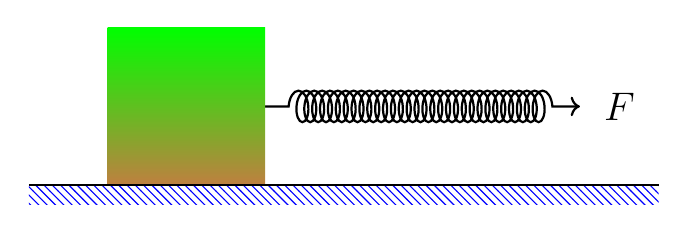
\begin{tikzpicture}
        %GRID
        %\draw[lightgray] (0,0) grid (5,5);

        %PEGAS
        \draw
        [
            thick, ->,
            decoration={
                coil,
                segment length = 1mm,
                amplitude = 2mm,
                aspect = 0.5,
                post length = 3mm,
                pre length = 3mm},
            decorate] (2,1) -- (6,1) node[right=5pt]{\Large $F$};
        
        %BALOK
        \shade[top color=green, bottom color=brown] (0,0) rectangle (2,2);

        %LANTAI
        \fill[pattern=north west lines, pattern color=blue] (-1,-0.25) rectangle (7,0);
        \draw[thick] (-1,0) -- (7,0);
    \end{tikzpicture}
\end{center}
    \begin{enumerate}
        \item $0,4 \; joule$
        \item $0,6 \; joule$
        \item $0,8 \; joule$
        \item $1,0 \; joule$
        \item $1,2 \; joule$
    \end{enumerate}

%20%
\item Sebuah elektron dan sebuah proton dengan kecepatan yang sama besarnya tetapi saling bertolak belakang, memasuki suatu wilayah bermedan magnet homogen. Rasio besar gaya yang dialami elektron terhadap yang dialami proton adalah \dots \\
\textbf{(Keterangan: $m_p$ dan $m_e$ adalah massa protaon dan massa elektron)}
    \begin{enumerate}
        \item $\frac{m_e}{m_p}$
        \item $\frac{m_p}{m_e}$
        \item $1$
        \item $\frac{2m_p}{m_e}$
        \item $\frac{1}{2}$
    \end{enumerate}

%21%
\item Kapasitas suatu kapasitor plat sejajar dapat dinaikan dengan \dots
    \begin{enumerate}
        \item Menaikan jumlah muatan
        \item Menurunkan jumlah muatan
        \item Menaikan jarak antar plat
        \item Menurunkan jarak antar plat
        \item Menurunkan luas plat
    \end{enumerate}
    
%22% 
\item Suatu $loop$ kawat berbentuk persegi empat dengan panjang sisi-sisi $0,3 \; m$ ditembus tegak lurus oleh medan magnetik luar $0,3 \; T$. Jika medan magnetik berubah arah dalam $1,5 \; s$ dan besarnya menjadi $0,2 \; T$, maka rata-rata ggl induksi dalam $loop$ kawat tersebut adalah \dots
    \begin{enumerate}
        \item $30 \; mV$
        \item $45 \; mV$
        \item $60 \; mV$
        \item $75 \; mV$
        \item $90 \; mV$
    \end{enumerate}
    
%23%
\item Sebuah kapal bermuatan bersandar di pelabuhan yang air lautnya tenang (tidak ada ombak). Ketika kapal dalam keadaan kosong tanpa muatan barang, akibat naik turunnya seorang kelasi dari kapal, kapal terayun-ayun naik turun terhadap permukaan air dengan periode ayunan $T_0$. Ketika kapal berisi muatan penuh, kapal terayun-ayun naik turun terhadap permukaan air dengan periode ayunan $T_1$. Rasio massa muatan kapal terhadap massa kapal ketika kosong kira-kira \dots
    \begin{enumerate}
        \item $\frac{T_0^2}{T_1^2}-1$
        \item $\frac{T_1}{T_0}-1$
        \item $\frac{T_1^2}{T_0^2}-1$
        \item $\frac{T_1^2}{T_0^2}$
        \item $\frac{T_0}{T_1}$
    \end{enumerate}
    
%24%  
\item Dua buah senar gitar yang panjangnya sama, gaya tegangan padanya sama tetapi massa totalnya berbeda mengalami peristiwa resonansi. Bila senar pertama bergetar pada nada dasarnya sedangkan senar kedua bergetar pada nada tingkat pertamanya, maka rasio massa senar pertama terhadap senar kedua adalah \dots
	\begin{enumerate}
		\item $4$
		\item $2$
		\item $1$
		\item $\frac{1}{2}$
		\item $\frac{1}{4}$
	\end{enumerate}
	
%25%
\item Sebuah teleskop memiliki pembesaran sebesar $20$ kali untuk mata yang tidak berakomodasi. Jika panjang teleskop adalah $84 \; cm$, maka panjang fokus lensa obyektif adalah \dots
   \begin{enumerate}
        \item $80 \; cm$
        \item $78 \; cm$
        \item $75 \; cm$
        \item $72 \; cm$
        \item $64 \; cm$
   \end{enumerate}
   
%26%
\item Berkas cahaya yang datang terhadap suatu medium dengan sudut sinar datang terhadap garis normal $30^\circ$ sebagian dipantulkan kembali ke udara dan sebagian lagi dibiaskan. Jika berkas sinar pantul dan berkas sinar bias saling tegak lurus satu dengan yang lain, maka indeks bias medium adalah sebesar \dots
    \begin{enumerate}
        \item $\sqrt{2}$
        \item $\frac{1}{\sqrt{2}}$
        \item $\sqrt{3}$
        \item $\frac{1}{\sqrt{3}}$
        \item $2$
    \end{enumerate}
  
%27%  
\item Sebuah lensa terbuat dari bahan dengan indeks bias $1,5$ memiliki jarak titik api $20 \; cm$ di udara. Lensa lain dengan geometri yang sama terbuat dari bahan yang indeks biasnya $1,4$. Berapakah jarak titik api lensa kedua ini?
    \begin{enumerate}
        \item $15 \; cm$
        \item $25 \; cm$
        \item $32 \; cm$
        \item $35 \; cm$
        \item $42 \; cm$
    \end{enumerate}
    
%28%  
\item Suatu gas ideal dengan volume $273 \; cm^3$ mula-mula bersuhu $20^\circ \; C$. Kemudian gas tersebut dipanaskan pada tekanan konstan hingga suhunya $30^\circ \; C$. Pertambahan volumenya adalah \dots
    \begin{enumerate}
        \item $10 \; cm^3$
        \item $20 \; cm^3$
        \item $30 \; cm^3$
        \item $40 \; cm^3$
        \item $50 \; cm^3$
    \end{enumerate}

%29%  
\item $150$ gram air pada gelas $A$ ingin deketahui suhunya dengan cara dicampur dengan air yang sudah diketahui suhunya. $100$ gram air dari gelas $A$ dicampur dengan air yang suhunya $48^\circ \; C$. Sisanya $50$ gram air dari gelas $A$ dicampur dengan $150$ gram air bersuhu $50^\circ \; C$. Ternyata suhu akhir kedua campuran tersebut sama. Asumsikan tidak ada kalor yang hilang ke udara maupun ke wadah air. Suhu air mula-mula pada gelas $A$ adalah \dots
    \begin{enumerate}
        \item $72^\circ \; C$
        \item $66^\circ \; C$
        \item $60^\circ \; C$
        \item $56^\circ \; C$
        \item $54^\circ \; C$
    \end{enumerate}

%30%
\item Dalam eksperimen efek fotolistrik, bila frekuensi cahaya yang digunakan sudah diatas ambang batas terjadinya efek fotolistrik, maka potensial penghenti akan memberikan energi \dots
    \begin{enumerate}
        \item Kinetik minimum elektron yang dapat lepas dari logam
        \item Potensial minimum elektron yang dapat lepas dari logam
        \item Kinetik maksimum elektron yang dapat lepas dari logam
        \item Potensial maksimum elektron yang tidak dapat lepas dari logam
        \item Potensial minimum elektron yang tidak dapat lepas dari logam
    \end{enumerate}
 
%31%
\item Usaha yang harus diberikan untuk menaikan kecepatan sebuah partikel bermassa $m$ dari $0,6 \, c$ menjadi $0,8 \, c$ adalah sebesar \dots
    \begin{enumerate}
        \item $\frac{10}{48} \; mc^2$
        \item $\frac{10}{24} \; mc^2$
        \item $\frac{10}{12} \; mc^2$
        \item $\frac{1}{24} \; mc^2$
        \item $\frac{1}{12} \; mc^2$
    \end{enumerate}

%32%
\item Suatu inti radioaktif $A$ memiliki waktu paruh $12$ jam. Jika pada suatu sampel yang pada saat awal berisi $m_0$ gram inti atom $A$, maka selama waktu $t=48$ jam hingga $t=60$ jam, banyaknya inti $A$ yang meluruh sebanyak \dots
    \begin{enumerate}
        \item $\frac{m_0}{32}$
        \item $\frac{m_0}{16}$
        \item $\frac{m_0}{8}$
        \item $\frac{m_0}{4}$
        \item $\frac{m_0}{2}$
    \end{enumerate}

%33%
\item Momentum suatu elektron awalnya sama dengan $mc$. Untuk memperkecil panjang gelombang de Broglie elektron ini agar menjadi setengah dari semula maka energi total elektron tersebut harus menjadi \dots
    \begin{enumerate}
        \item $\sqrt{2} \; mc^2$
        \item $\sqrt{3} \; mc^2$
        \item $\sqrt{4} \; mc^2$
        \item $\sqrt{5} \; mc^2$
        \item $\sqrt{6} \; mc^2$
    \end{enumerate}

%34%
\item Suatu partikel dengan massa diam $m$ memiliki momentum $\sqrt{0,44} \; mc$. Energi kinetik dari partikel ini adalah \dots
    \begin{enumerate}
        \item $0,5 \; mc^2$
        \item $0,4 \; mc^2$
        \item $0,3 \; mc^2$
        \item $0,2 \; mc^2$
        \item $0,1 \; mc^2$
    \end{enumerate}

%35%
\item Dua buah satelit $M$ dan $N$ masing-masing mengitari planet $P$ yang berbentuk bola pada ketinggian berturut-turut $1000 \; km$ dan $6000 \; km$ dari permukaan planet tersebut. Periode satelit $M$ dan $N$ berturut-turut $8$ jam dan $27$ jam. Jari-jari planet P tersebut adalah \dots
    \begin{enumerate}
        \item $1000 \; km$
        \item $2000 \; km$
        \item $3000 \; km$
        \item $4000 \; km$
        \item $6000 \; km$
    \end{enumerate}

\end{enumerate}
\end{document}  
